
\begin{frame}
    \frametitle{\normalsize \textbf{Естественность полей, колец и тел}}
    \framesubtitle{Дополнение к дальшейшим слайдам}
    Всем известно такое понятие, как <<множество>>. В общем случае, элементами множества могут являться любые элементы (например, слоны), однако хочется подойти к этому понятию с другой стороны, рассмотреть его свойства более подробно и в более частных случаях. Именно поэтому выделяют особые типы множеств: \textcolor{blue}{\it кольца (коммутативные, с единицей), тела, поля}. Дальше мы введём аксиомы для них и будем изучать их свойства, различные поля и кольца, выделять более частные типы колец (полей), и тому подобное.

\end{frame}

\includepdf[pages=2]{0_basic}

\begin{frame}[t]
    \frametitle{\normalsize \bf Примеры}
    Легко видеть, что поле -- это частный случай кольца.
    
    $\Z$ --- кольцо, но не поле (нет обратных элементов по $\cdot$).
    
    $\R$ -- поле.

    $\N$ -- ни кольцо, ни поле (нет обратных по $+$).
     
    <<Множество дробей>> -- поле (мы это докажем).


    Докажем некоторые свойства колец и полей. Это будет делаться так: либо мы предполагаем противное и доказываем, что тогда эти 2 числа равны, либо из левой части того, что нужно доказать в результате операций получаем правую часть утверждения (или комбинируя).
\end{frame}

\includepdf[pages=3-5]{0_basic}

\begin{frame}[t]
    \frametitle{\normalsize \bf Подполе и подкольцо}
    \small
    \begin{block}{Определение}
        \begin{itemize}
            \item Пусть $K \subset L$, причем оба они — кольца с одними и
теми же операциями $+$ и $\cdot $. Тогда $K$ — подкольцо $L$, а $L$
— надкольцо $K$ .
    \item  
 Пусть $K \subset L$, причем оба они — поля с одними и теми
же операциями $+$ и $\cdot $. Тогда $K$ — подполе $L$, а $L$ —
надполе $K$.
        \end{itemize}
    \begin{wrapfigure}{r}{0.4\textwidth}
        \centering
        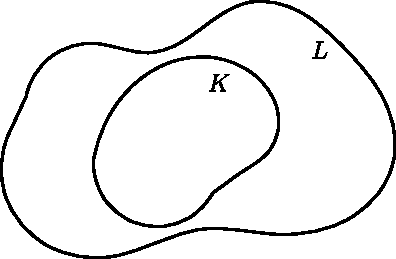
\includegraphics[width=0.4\textwidth]{images/path1}
        \label{fig:path1}
    \end{wrapfigure}
    
    У подкольца все свойства операций \textcolor{red}{наследуются}.

    Верное определение $+, \cdot \iff$ замкнутость по $+, \cdot $. 

    В следующих утверждениях мы просто проверим условия для кольца/поля. 
\end{block}

\end{frame}

\includepdf[pages=7-8]{0_basic}
\begin{frame}[t]
    \frametitle{\normalsize \bf Естественность гомоморфизма}
    \framesubtitle{Дополнение к дальшейшим слайдам}
    \begin{definition}[Отображение]
        \small
        \textcolor{blue}{Отображение} $f: X \mapsto Y$ -- это правило, удовлетворяющее следующему утверждению: $\forall x \in X \exists y \in Y: f(x) = y$.
    \end{definition}

    \textcolor{blue}{Гомоморфизм} $f: K \mapsto L$ -- это отображение, которое как бы сохраняет структуру одного множества в другом. Оперируя над числами с помощью этого отображения, мы не можем получить, например, что $f(2) = 3$. 

    \begin{figure}[h]
        \centering
        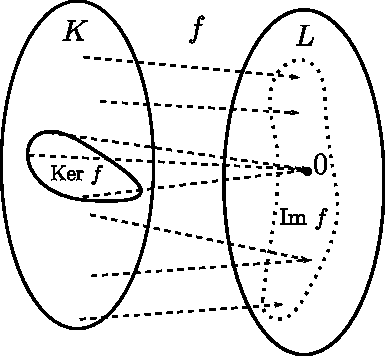
\includegraphics[width=0.35\textwidth]{images/path2}
        \label{fig:path2}
    \end{figure}

\end{frame}
\includepdf[pages=9]{0_basic}
\begin{frame}[t]
    \setcounter{lemma}{2}
    \begin{lemma}[Критерий кольца]
        Пусть $K , L$ — кольца, $f : K \mapsto  L$ --- гомоморфизм колец.
        Тогда:
        \begin{enumerate}
            \item $\ke (f )$ --- подкольцо $K$.
            \item $\im(f )$ --- подкольцо $L$.
        \end{enumerate}
    \end{lemma}

    \begin{proof}[Доказательство]
        \renewcommand{\qedsymbol}{}
        Очевидно, что $\ke (f) \subset K$ и $\im (f) \subset L$. Тогда остаётся проверить замкнутость, наличие обратного элемента (Лемма 1).
        \begin{enumerate}
            \item Пусть $a,b \in \ke (f)$ $ \Rightarrow f(a)f(b) = 0 = f(ab) \Rightarrow $ $\Rightarrow ab \in \ke (f), $ (получилось, что  $f(ab) = 0 \Rightarrow$ по определению ядра $ab \in \ke (f)$)
                $f(a+b) = f(a) + f(b) = 0 + 0 = 0 \Rightarrow a+b \in \ke (f)$
            Пусть $x \in \ke f \Rightarrow 0 \overset{0 = f(0)} = f(x + (-x)) = f(x) + f(-x) = 0 + f(-x) = f(-x)$ 
        \end{enumerate}
    \end{proof}
\end{frame}

\begin{frame}[t]
    \framesubtitle{Окончание}
    
    \begin{enumerate}
        \setcounter{enumi}{1}
        \item Пусть $x,y \in \im (f)$. Тогда существуют элементы $x', y' \in K: f(x') = x, f(y') = y$. Итак, $x + y = f(x') + f(y') = f(x' + y') \Rightarrow x + y \in \im (f)$
            $xy = f(x')f(y') = f(x'y') \Rightarrow xy \in \im (f)$
            
            \vspace{0.2cm}
            Пусть $a \in \im (f)$. Тогда $\exists a': f(a') = a \Rightarrow -f(a') = -a$ $ \Rightarrow 0 - f(a') = -a \Rightarrow f(0 - a') = -a \Rightarrow f(-a') = -a \Rightarrow -a \in \im f$,\hfill \qedsymbol{}
    \end{enumerate}

    \begin{figure}[h]
        \centering
        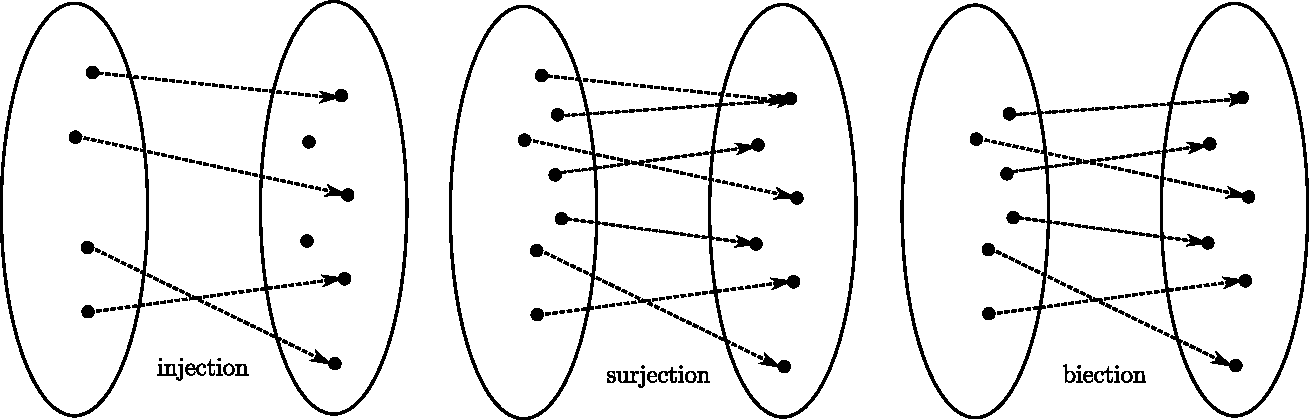
\includegraphics[width=\textwidth]{images/path3}
        \label{fig:path3}
    \end{figure}
\end{frame}

\begin{frame}[t]
    \frametitle{\normalsize \bf Критерий мономорфизма}
    \framesubtitle{Типы гомоморфизмов}
    \begin{itemize}
        \item 
        Если $f$ -- инъекция, то $f$ -- мономорфизм.

        \item  
        Если $f$ -- сюръекция, то $f$ -- эпиморфизм.
        
        \item  
        Если $f$ -- биекция, то $f$ -- изоморфизм.
    \end{itemize}

    \setcounter{lemma}{3}
    \begin{lemma}[Критерий мономорфизма]
        $f: K \mapsto  L $ -- мономорфизм $\iff \ke f = \left\{ 0 \right \}  $
    \end{lemma}

    \begin{proof}[Доказательство]
        \fbox{$ \Rightarrow $} Пусть это не так. Тогда $\left\{ 0, a \right \}  \subset \ke f$, но $f$ -- инъекция, и 2 элемента множества не могут отображаться в 1 элемент!?
        
        \fbox{$ \Leftarrow $} Проверим инъекцию (она всегда так проверяется): $f(x) = f(y) \Leftrightarrow f(x - y) = 0 \overset{\ke f = \left\{ 0 \right \} } \iff x - y = 0 \Leftrightarrow x = y$
    \end{proof}
    
\end{frame}

\begin{frame}[t]
    \frametitle{}
    \framesubtitle{}

    \begin{lemma}
        Пусть $f: K \mapsto L$ -- изоморфизм колец. Значит, $f^{-1}: L \mapsto K$ тоже является изоморфизмом.
    \end{lemma}

    \begin{proof}[Доказательство]
       Понятно, что $f^{-1}$ -- это биекция (если мы отобразили в $L$, то может и отобразить обратно, т. к. это биекция). Значит, остаётся проверить гомоморфизм. Для этого будем пользоваться тем, что  $f$ -- гомоморфизм.

    \end{proof}
\end{frame}

\includepdf[pages=12-33]{0_basic}
